%%%%%%%%%%%%%%%%%%%%%%%%%%%%%%%%%%%%%%%%%%%%%%%%%%%%%%%%%%%%%%%%%%%%%%%%%%%%%%
\documentclass[12pt,hidelinks]{article}

% 1. Load LaTeX packages
\usepackage{fontspec}
\usepackage{geometry}
\usepackage{lastpage}
\usepackage{fancyhdr}
\usepackage{hyperref}
\usepackage{amsmath}
\usepackage{amsthm}
\usepackage{xunicode}
\usepackage{listings}
\usepackage{color}
\usepackage{amssymb}

% 2. Define page dimensions and spacing
\geometry{top=1in, bottom=1in, left=1in, right=2in, marginparsep=4pt,
          marginparwidth=1in}
\setlength{\parindent}{0pt}
\setlength{\parskip}{12pt}

% 3. Set header, footer, and bibliography
\renewcommand{\headrulewidth}{0pt}
\pagestyle{fancyplain}
\fancyhf{}
\lfoot{}
\rfoot{page \thepage\ of \pageref{LastPage}}
\bibliographystyle{acm}

% 4. Set fonts for the document
\defaultfontfeatures{Mapping=tex-text}
\setromanfont{YaleNew}

% 5. Define custom code for book environments and commands
\DeclareMathOperator*{\argmin}{arg\,min}
\DeclareMathOperator*{\argmax}{arg\,max}
\newcommand{\code}[1]{\texttt{#1}}
\newcommand{\pkg}[1]{\textbf{#1}}

% 6. Define custom code for book environments and commands
\definecolor{verbgray}{gray}{0.9}
\definecolor{verbgray2}{gray}{0.975}

\lstnewenvironment{rcode}{%
  \lstset{backgroundcolor=\color{verbgray},
  frame=single,
  framerule=0pt,
  basicstyle=\ttfamily,
  keepspaces=true,
  columns=fullflexible}}{}

\lstnewenvironment{rres}{%
  \lstset{backgroundcolor=\color{verbgray2},
  frame=single,
  framerule=0pt,
  basicstyle=\ttfamily,
  keepspaces=true,
  columns=fullflexible}}{}

% 7. Define numbering scheme for equations (only needed for handout).
\numberwithin{equation}{section}
\setcounter{section}{1}

%%%%%%%%%%%%%%%%%%%%%%%%%%%%%%%%%%%%%%%%%%%%%%%%%%%%%%%%%%%%%%%%%%%%%%%%%%%%%%
\begin{document}

{\LARGE Handout 04: Normal Equations}

\vspace*{18pt}


\section{Ordinary least squares}

\index{ordinary least squares}
Many of the advantages of linear models concern the beneficial properties
of the standard estimators used to compute the unknown parameters
$\beta_j$ from observed data. As a next step we would like to explore
the definition of these estimators. To this aim, it will be useful to
provide a compact matrix-based description of a linear model. Throughout
this text, unless otherwise noted, we use a notation where $n$ is the
sample size, $p$ is the number of variables, $i$ is an index over the
samples, and $j$ is the index over the variables. With this notation a
complete general description of a linear model can be given by
\begin{align}
y_i &= \beta_1 \cdot x_{i,1} + \cdots + \beta_p \cdot x_{i,p} + \epsilon_i, \quad \forall\,  i = 1, \ldots, n.
\end{align}
Or simply
\begin{align}
y_i &= \sum_j \beta_j \cdot x_{i,j} + \epsilon_i, \quad \forall\,  i = 1, \ldots, n.
\end{align}
Notice that we do not need to include an explicit intercept term
$\beta_0$. If one is required this can be included by setting
$x_{i,1}$ equal to one for every single observation $i$. Using
matrix notation, we can write the linear model equation
simultaneously for all observations as
\begin{align}
\left(\begin{array}{c}y_1\\ y_2\\ \vdots\\ y_n\end{array}\right) &=
  \left(\begin{array}{cccc}x_{1,1}&x_{2,1}&\cdots&x_{p,1}\\
                           x_{1,2}&\ddots&&x_{p,2}\\
                           \vdots&&\ddots&\vdots\\
                           x_{1,n}&x_{2,n}&\cdots&x_{p,n}\\\end{array}\right)
  \left(\begin{array}{c}\beta_1\\ \beta_2\\ \vdots\\ \beta_p\end{array}\right) +
  \left(\begin{array}{c}\epsilon_1\\ \epsilon_2\\ \vdots\\ \epsilon_n\end{array}\right)
\end{align}
which can be compactly written in terms of a vector $y$ of the responses,
a matrix $X$ of the predictor variables, a vector $\beta$ of the unknown
parameters, and a vector $\epsilon$ of the errors
\begin{align}
y &= X \beta + \epsilon.
\end{align}
Beyond compactness, this notation is also useful as many of the computational
properties of linear models can be reduced to linear algebraic properties of
the matrix $X$.

\index{residual vector}
It is desirable for an estimate $\widehat{\beta}$ of the unknown vector $\beta$
to be able to explain as much variation as possible of the responses $y$. One way
of viewing a linear model is as a decomposition of $y$ into a fixed, deterministic
signal $X\beta$ and a stochastic random noise term $\epsilon$. Prediction and
inference both benefit from making the signal term as dominant as possible. A
good method for measuring this is to construct the vector of residuals
\begin{align}
r &= y - X\widehat{\beta}.
\end{align}
We can compare estimators by comparing the size of their residual vectors.
A graphical representation of residuals from a linear model is given in
Equation~\ref{lm_residuals}.

\begin{figure}
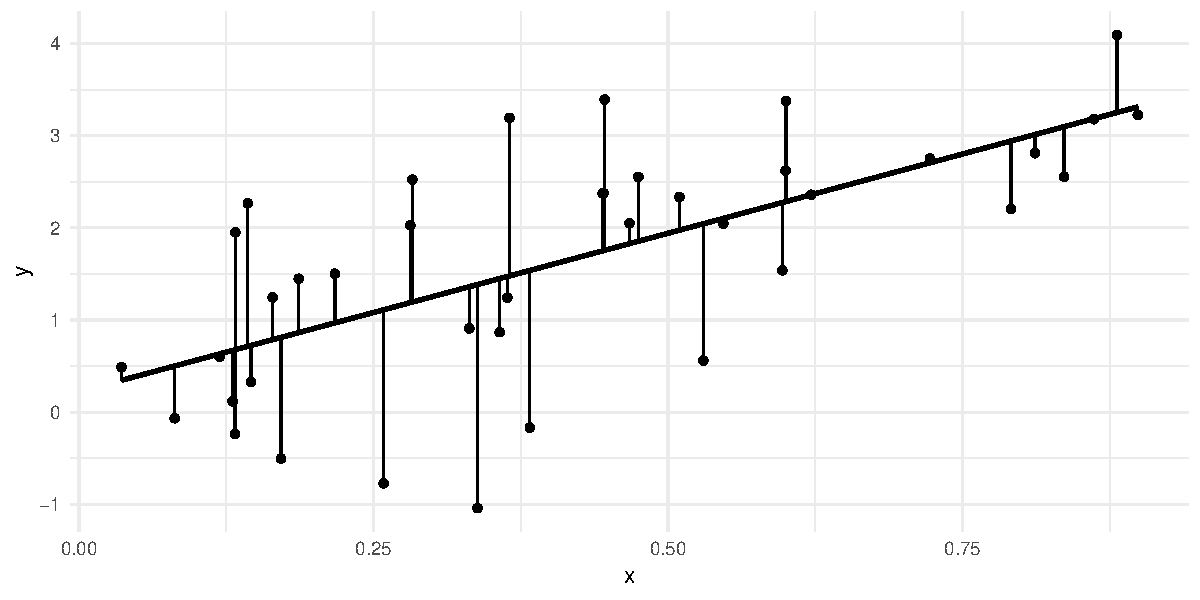
\includegraphics[width=\textwidth]{figures/lm_residuals.pdf}
\caption[Residuals from a simple linear model]{Visualization of residuals
from the linear model $y = \beta_0 + \beta_1 x$.}
\label{lm_residuals}
\end{figure}

There are many choices for measuring the size of a regression vector,
several of which lead to important, and distinct, estimators. The hinged loss,
which penalizes positive residuals more than negative ones (or vice versa),
leads to quantile regression.
Metrics that penalize all residuals past some large threshold equally lead
to robust regression techniques. Metrics
that give each sample a weight $w_i$ depending on the specific values of the
data $x_i$ can result in kernel regression (Section~\ref{sec_kernel_reg}),
local regression (Section~\ref{sec_local_reg}) and are an important
intermediate step in solving the generalized linear model problems that
arise in Chapters~\ref{ch_glm}, \ref{ch_additive}, and \ref{ch_glmnet}.

In this chapter, we will focus on the most popular choice of metric to
measure the size of the regression vector: the sum of squared residuals.
Minimizing the sum of squared residuals leads to the %ubiquitous
\textit{ordinary least squares} (OLS) estimator. Why is this such a
popular choice? For one thing, it allows us to write the metric in terms
of an inner product or vector norm
\begin{align}
\sum_i r_i^2 &= r^t r = || r ||_2^2,
\end{align}
a form that is easy to work with both computationally and theoretically.
The choice of the sum of squared residuals is also motivated by
the maximum likelihood estimator when the $\epsilon_i$'s are independent
and identically distributed random variables with a normal distribution
having zero mean.

\section{The normal equations}

\index{normal equations}
We now have a formal specification of the ordinary least squares
estimator. Computing the estimator given a set of observed data
requires solving an optimization problem. This particular optimization
problem is unconstrained and has a continuous gradient, so an
obvious first step would be to find the gradient of the least
squares objective function with respect to the vector $b$
\begin{align}
\nabla_b \left[ || y - X b ||_2^2  \right] &= \nabla_b \left[ y^t y + b^t X^t X b - 2 y^t X b \right] \\
&= 2 X^t X b - 2 X^t y. \label{normalish_equations}
\end{align}
A necessary condition for minimizing the objective function is to have
the gradient equal to the zero vector, $\vec{0}$. If the Hessian matrix
is positive definite at this solution, only then are we guaranteed to have a
local minimum. The Hessian matrix here is constant everywhere, in
that it does not depend on the value of $b$. Specifically, it is
given by
\begin{align}
H\left( || y - X b ||_2^2  \right) &=  X^t X.
\end{align}
For a matrix $M$ to be positive definite, we need to have $z^t M z$ be
strictly positive for any vector $z$ not equal to the zero vector.
Notice that in our case this matrix product can be written as a
vector norm
\begin{align}
z^t H\left( || y - X b ||_2^2  \right) z &=  z^t X^t X z \\
&= || X z ||_2^2.
\end{align}
The squared $\ell_2$-norm is never negative and is only zero at the
zero vector.

\index{Hessian matrix}
We see then that the Hessian is positive definite everywhere if
and only if a non-zero vector $z$ does not exist such that $Xz$
is the zero vector. This, in turn is true if and only if $X$ is not
full rank. In this case, there are many possible values of $b$ that
all attain the minimum least squares solution. Such a result should
not surprise us. If we have such a $z$, then there are many parameter
vectors $b$ that result in the exact same estimates for $y$ as there
are for the true $\beta$
\begin{align}
X (\beta + a \cdot z) &= X \beta + a X z \\
&= X \beta + \vec{0} \\
&= X \beta.
\end{align}
In such cases it is
possible to place constraints on the problem to formulate a related
problem with a unique solution. For instance, Section~\ref{sec_ols_svd}
illustrates how to find the unique OLS solution of minimal norm.
Although minimum-norm least squares solutions are widely used in many science
and engineering applications, it is more common in statistics to constrain
solutions to rank-deficient problems in other ways. In particular, R's
\code{lm} and \code{glm} solvers reformulate rank-deficient problems into
full-rank ones by selecting a subset of columns using a heuristic procedure
based on the model matrix column order. Other common subset selection
approaches include the lasso (see Chapter~\ref{ch_glmnet}), which solves a
penalized version of OLS.

%In this case even if the noise vector $\epsilon$ is not present, we
%still will not be able to accurately compute $\beta$. It therefore seems
%justifiable that we assume, for now, that $X$ is a full column rank
%matrix.

Satisfied that we attain a local minimum wherever the gradient is zero,
we return to Equation~\ref{normalish_equations}. Setting this
equal to zero we get what are known as the \textit{normal equations},
a linear system of equations of $p$ variables over $p$ unknowns
expressed in matrix form as
\begin{align}
X^t X b &= X^t y. \label{norm_eq}
\end{align}
Solving systems like the normal equations for $b$ in a numerically stable and
efficient manner is an important problem encountered repeatedly in this text.
Linear systems of equations are generically solved by Gaussian
elimination, but we will see that other more efficient and/or numerically
stable methods based on the Cholesky, QR, or SVD decompositions can be
used depending on context.



\renewcommand{\section}[2]{}%
\vspace{12pt}
\textbf{References}
\bibliography{bibfile}

%%%%%%%%%%%%%%%%%%%%%%%%%%%%%%%%%%%%%%%%%%%%%%%%%%%%%%%%%%%%%%%%%%%%%%%%%%%%%%
\newpage

\textbf{LAB QUESTIONS}

\vspace*{0pt}

\begin{enumerate}
\item Here is a thing!
\end{enumerate}

\end{document}

